\section{Continuous Integration}

\subsection{Understanding Continuous Integration}

Continuous Integration (CI) is a development practice where developers frequently integrate their code into a shared repository.
Each integration is then automatically checked by an automated build, this will allow teams to detect problems early and thereby use less time trying to bug fix
and error locate doing development.

In our context, CI gives os the opportunity to do rapid development of our software by ensuring that new code changes do not break existing functionalities of the program when
we push refactored code to the development branch.
CI works by doing a series of automated tests and builds, this is triggered when developers push code to the repository ensuring code quality and stability when multiple
developers are working simultaneously on the program.

\subsection{Continuous Integration Implementation}
For our project, CI is implemented using GitHub Actions, which is a tool on github that allows developers to do CI/CD which will automates our build and test processes.
Our pipeline, defined in the .github/workflows directory, specifies the actions to be taken when a pull request is made to the develop branch.

The pipeline is composed of several steps, each step is a job that is run on a virtual machine hosted by GitHub.

\textbf{Checkout:} Retrieves the code from the repository.

\textbf{Set up JDK 11:} Configures the Java Development Kit, version 11, which is necessary for building and testing Java applications.

\textbf{Build with Maven:} Compiles the project, skipping the tests for speed in this initial phase, using Maven - a software project management tool.

\begin{figure}[H]
    \centering
    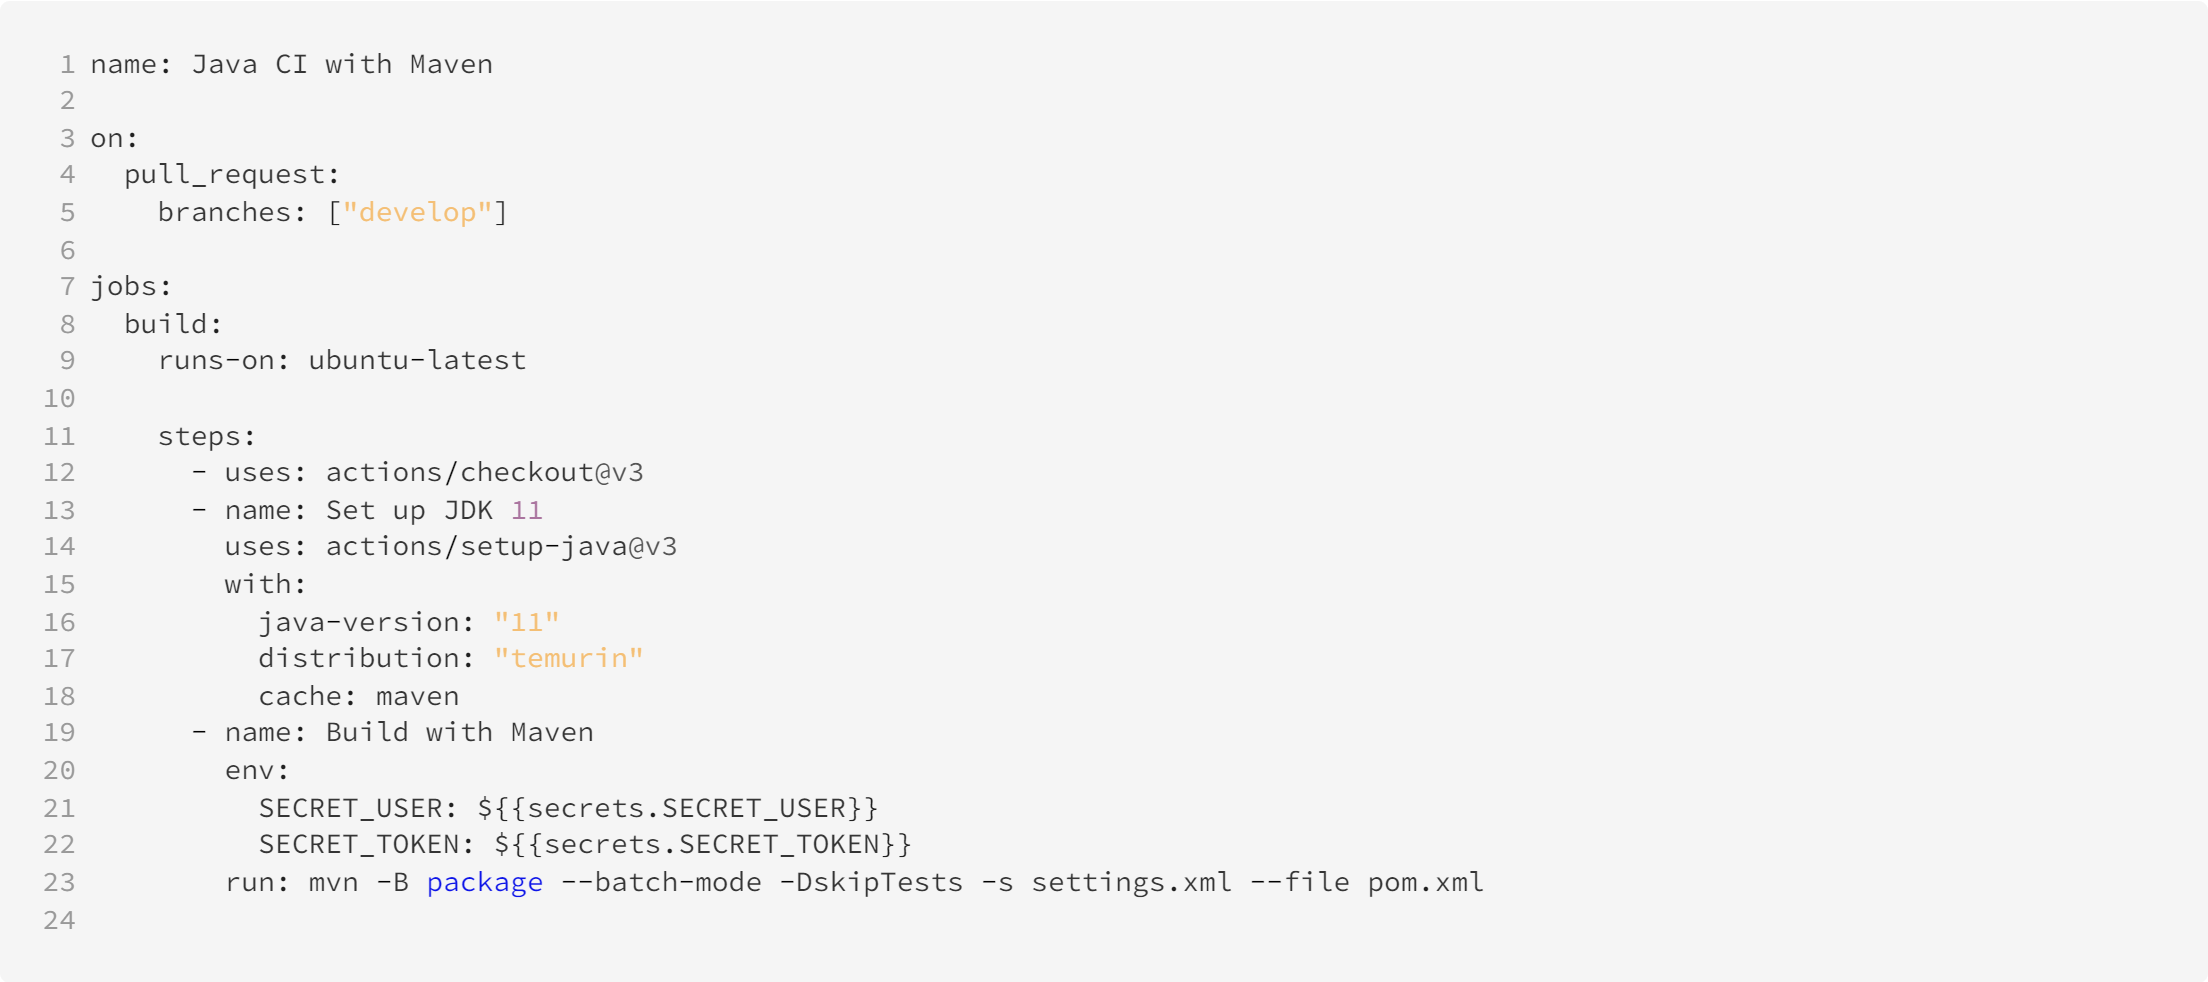
\includegraphics[width=\linewidth]{pic/Continuous Integration yml file.png}
    \caption{Continuous Integration yml file}
    \label{fig:Continuous Integration yml file}
\end{figure}

By using Integrating CI in our development process it gives us several benefits such as.

\textbf{Early Bug Detection:} Bugs and integration issues are detected and fixed early in the development cycle, since we will be alerted sooner.

\textbf{Rapid Feedback:} Developers will receive instant feedback on their code, speeding up the development and review process immensely.

\textbf{Consistent Code Quality:} Automated tests ensure code quality is maintained by all developers, reducing the chance of introducing new bugs or erros unknowingly.

\textbf{Enhanced Collaboration:} Promotes collaboration among team members, as CI will ensure that the code in the repository is always in a stable state and running correctly.

\subsection{Version Control with Git}

Our project uses Git, which is a distributed version control system, to manage any changes to the codebase that developers on the project might make.
Git allows multiple developers to work on the same codebase simultaneously, without overwriting each other's changes.

In our project we started by baching out from main to a develop branch, this was done to ensure that the main branch always contains a stable version of the codebase. From the develop branch we could then branch out into our
own feature branches, where we could work on our own features without affecting the develop branch. When we were done with our feature, we could then merge our feature branch
into the develop branch, where it would be reviewed before being merged into the main branch by the ind of the project, when the delevop branch had a stable running build.